\documentclass[a4paper]{article}

\usepackage{a4wide,times}
\usepackage[english]{babel}
\usepackage[utf8]{inputenc}
\usepackage{listings}
\usepackage{color}
\usepackage{graphics}
\usepackage{ragged2e}
\usepackage{graphicx}
\usepackage{geometry}
\usepackage{marginnote}
\usepackage{enumitem}
\usepackage{hyperref}
\usepackage{verbatim}

\definecolor{codegreen}{rgb}{0,0.6,0}
\definecolor{codegray}{rgb}{0.5,0.5,0.5}
\definecolor{codepurple}{rgb}{0.58,0,0.82}
\definecolor{backcolour}{rgb}{0.95,0.95,0.92}
 
\lstdefinestyle{mystyle}{
    backgroundcolor=\color{backcolour},   
    commentstyle=\color{codegreen},
    keywordstyle=\color{blue},
    numberstyle=\tiny\color{codegray},
    stringstyle=\color{codepurple},
    basicstyle=\footnotesize,
    breakatwhitespace=false,         
    breaklines=true,                 
    captionpos=b,                    
    keepspaces=true,                 
    numbers=left,                    
    numbersep=5pt,                  
    showspaces=false,                
    showstringspaces=false,
    showtabs=false,                  
    tabsize=2
}
 
\lstset{style=mystyle}

\begin{document}


\title{Object Oriented Programming\\
Final Project Report \\
Graph Editor
}

\date{\today}

\author{First Author \quad Second Author\\
Andr\'es Salinas Lima (S3837416) \quad Russell Sammut-Bonnici (S3839397)
}

\maketitle



\section{Problem Description}
\par The task at hand is to create an undirected graph editor with a graphical user interface in Java. It should be designed using Swing and Java IO, with the MVC (Model-View-Controller) architectural pattern kept in mind. The MVC approach is important in order to keep the reasonably complex code maintainable. 
\par Using the keyboard and/or mouse the user should be able to edit graphs as well as save and load them. The input behaviour should be keyboard/mouse signals received from the user, which should in turn activate actions when detected. The output behaviour should emerge from the activated actions and result in observable changes in the graph.



\section{Problem Analysis}
\par The graph editor can be thought of in two parts. The first part is the graph itself; what it consists of, how it can be interpreted during saving and loading, and so on. The second part is the editor; how the structural information of the graph is utilized, how the graph is displayed and what actions the user can impose on the graph.

\subsection{The Graph} \label{par: The Graph}
\par A graph model is described as a composition of vertices and edges. A vertex is represented by a rectangle, with its own name, size and location. An edge is represented by a line that connects one vertex to another. The pair is unordered in this case as the graph is undirected.

\subsection{The Editor}
\par The Editor is the graphical interface that will allow the user to interact (visualize and modify) with the graph. Though simplistic of a concept, this is worth mentioning as much of the program's code has to follow this graph-editor separation for clarity. 
\par The editor is represented by a window, composed of a frame and a panel. The structural information of the graph model is called at this level for presentation in the panel. The user can edit, open, save or create the graph model through actions accessed through buttons, menu items and keyboard shortcuts.



\section{Program Design}
\par This program was designed with the MVC architectural pattern kept in mind. Tackling from these three aspects makes the problem much more approachable as well as the program in itself more maintainable and secure. 
\par More maintainable because the approach is modular. When something goes wrong in one section, it is easily identifiable from which section the issue is stemming from. More secure because having to call classes from outside their packages motivates encapsulation, where secure getters and setters are the only way to  interpret and redefine instantiated objects.
\par Source code files were structured through packages according to model-view-controller as seen in Figure \ref{fig: PackageDiagram} below. A brief description of each part will be given in this section. \\

\begin{figure}[h!]
    \centering
    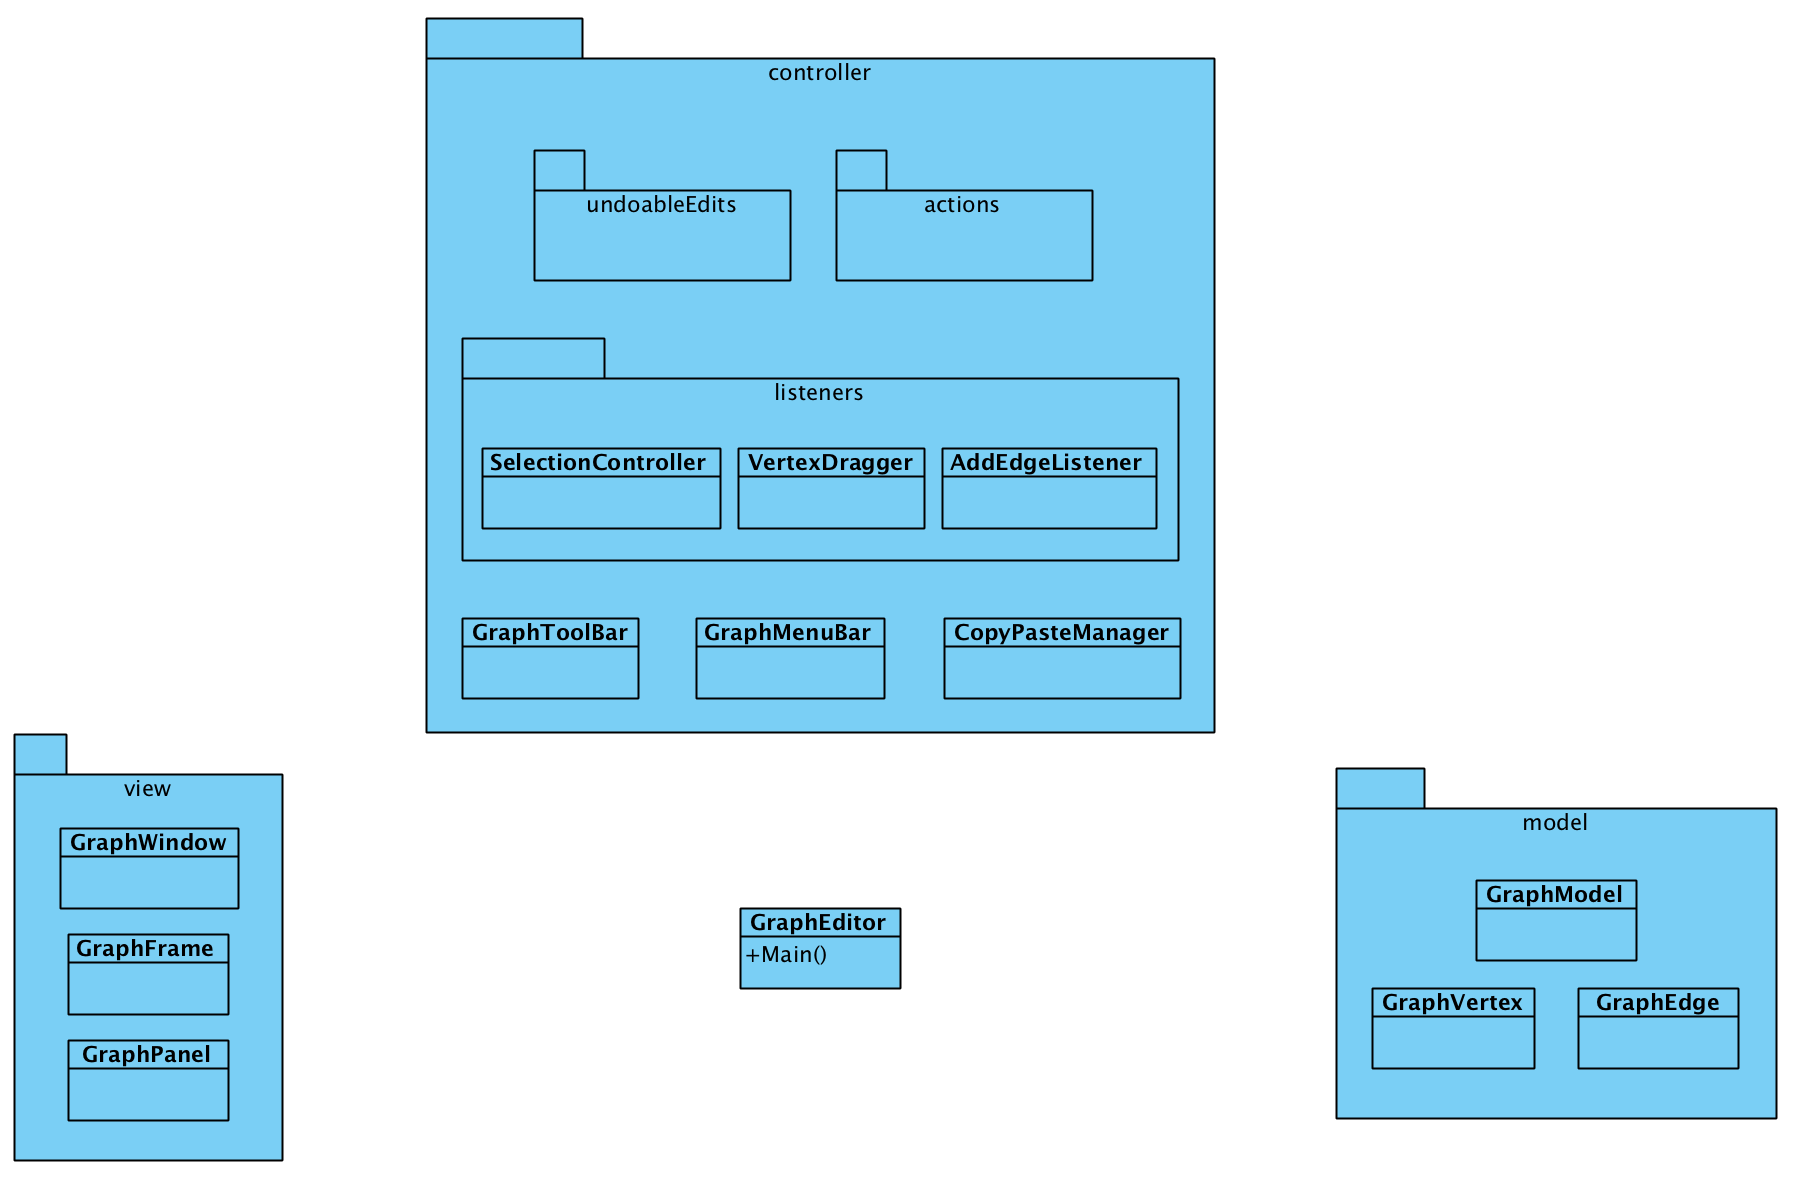
\includegraphics[width=0.9\textwidth]{im/PackageDiagram.png}
    \caption{Package diagram}
    \label{fig: PackageDiagram}
\end{figure}

\subsection{Model}
\par The Model is the graph structure described in section \ref{par: The Graph}, which is implemented by the \textit{GraphModel}, \textit{GraphVertex} and \textit{GraphEdge} classes. The graph components are essentially implemented by an\\ \textit{ArrayList$<$GraphVertex$>$} for vertices and an  \textit{ArrayList$<$GraphEdge$>$} for edges, with selected vertices and edges kept track of by two additional object ArrayLists. 
\par \textit{GraphModel} could be considered the most important class of this program, as it's on charge of modifying the graph, keeping track of the changes made to its vertices and notifying the view of all these changes. This was easy to make thanks to the observer design pattern and the already implemented \textit{Observable} class and \textit{Observer} interface of Java. In addition to that, the \textit{GraphModel} is also the place where the \textit{UndoManager} and the \textit{CopyPasteManager} reside.
\par A class diagram of the Model is shown in Figure \ref{fig: Model}.

\begin{figure}[h!]
    \centering
    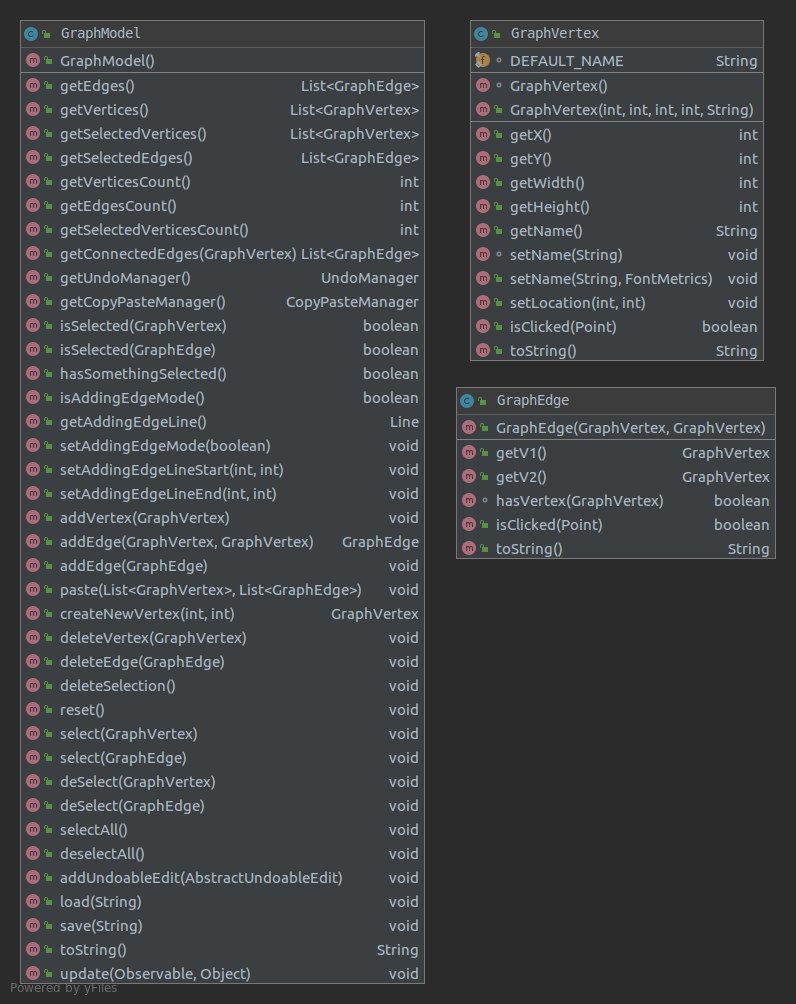
\includegraphics[width=0.7\textwidth]{im/Model.png}
    \caption{Graph Model}
    \label{fig: Model}
\end{figure}

\subsection{View}
\par The View is the window composed of the frame and panel as well as the presentation of the model within the panel: \textit{GraphWindow} contains the \textit{GraphFrame} which contains the \textit{GraphPanel} inside of a \textit{ScrollPane} which allows the user to scroll the panel. All the painting work is done in the \textit{GraphPanel} class for graph model display (Figure \ref{fig: mvc}). When the graph model is modified, via the observer design pattern, the \textit{GraphPanel} gets notified and repaints the panel to display the updated model.

\subsection{Controller}
\par The Controller generally consists of the Menu Bar (\textit{GraphMenuBar} class), the Tool Bar  (\textit{GraphToolBar} class), the actions for both the Menu and Tool Bars  (\textit{actions} package), the mouse and keyboard listeners ( (\textit{listeners} package with the \textit{AddEdgeListener}, \textit{SelectionController} and \textit{VertexDragger} classes) and all the undoable edits for the model (\textit{undoableEdits} package) that will be managed by the UndoManager.
\par Since the functionality of the class \textit{CopyPasteManager} is an extension of the program it is later explained in section \ref{section: extension}. On the other hand, the \textit{GraphToolBar} isn't an extension but it isn't necessarily essential either. Its purpose is user-friendliness. It basically provides the user with easy access to the frequently used actions; new graph, open, save, undo, redo, add vertex, add edge, rename vertex, select all and delete selection. The same actions, alongside more complex actions, can be easily accessed via menu items in the \textit{GraphMenuBar}. It's organised as follows:

\subsubsection{The Graph Menu Bar} 
\marginnote{\footnotesize Note that each of the menu items (apart from Show Toolbar and Default Size) have keyboard shortcuts assigned to them, which are further discussed in section \ref{section: Keyboard Shortcuts}.}[1cm]
\begin{enumerate}
    \item \textbf{File}
        \begin{enumerate}[label*=\arabic*.]
            \item \textbf{New Graph}: Simply resets the graph by deleting all of its vertices and edges
            \item \textbf{Open}: Loads a graph from a .txt file.
            \item \textbf{Save}: Saves the current graph as a .txt file.
            \item \textbf{Quit}: Exits the program.
        \end{enumerate}
    \item \textbf{Edit}
        \begin{enumerate}[label*=\arabic*.]
            \item \textbf{Undo}: Undoes the user's most recent edit.
            \item \textbf{Redo}: Reverts the previous undo action.
            \item \textbf{Copy}: Copies the selected vertices (and edges between them).
            \item \textbf{Cut}: Cuts the selected vertices (and edges between them).
            \item \textbf{Paste}: Pastes the copied/cut vertices and edges.
            \item \textbf{Add Vertex}: Adds a new vertex to the graph with the default name in the default position but when added, its name and position will be adjusted if they conflict with already existing vertices. New vertices will always appear in the top left corner.
            \item \textbf{Add Edge}: Creates a new edge from the selected vertex. A new line is drawn from the selected vertex to the user's cursor (Figure \ref{fig: addE}). When a user selects another vertex an edge is created between those two vertices, otherwise (if something else is selected in the panel) the line is removed and no edge is added. An edge cannot be created between two vertices if there already exists (Figure \ref{fig: edgePopUp}). An edge can't be made from a vertex to itself (Figure \ref{fig: edgeSelfLoop}).
            \item \textbf{Rename Vertex}: Renames the selected vertex (Figure \ref{fig: ren}). Multiple vertices cannot be renamed (Figure \ref{fig: ErrorRen}).
            \item \textbf{Select All}: Selects all the vertices and edges.
            \item \textbf{Delete Section}: Removes any selected vertices and edges from the graph.
        \end{enumerate}
    \item \textbf{Window}
        \begin{enumerate}[label*=\arabic*.]
            \item \textbf{Show Toolbar} Initially set to visible, it toggles the visibility of the GraphToolBar  (Figure \ref{fig: tog}).
            \item \textbf{New Window}: Creates a new window with a new graph.
            \item \textbf{Duplicate Window}: Creates a new window but with the current graph. All the windows containing the same graph will update in real time.
            \item \textbf{Default Size}: It simply resets the window back to its initial default size.
        \end{enumerate}
\end{enumerate}



\section{Extensions of the Program} \label{section: extension}

\subsection{Keyboard Shortcuts} \label{section: Keyboard Shortcuts} 
\par The keyboard shortcuts were mapped to their respective menuItem in the GraphMenuBar. This was done by calling \textit{setAccelerator()} from the extended class JMenuBar. Inside the parameters we fed the keystroke of the keyboard shortcut to be assigned. The keystroke was obtained using \textit{KeyStroke.getKeyStroke()}. 
\begin{table}[h!]
    \centering
    \begin{tabular}{c|c||c}
         \hline
         Menu name & Action name & Keyboard shortcut\\
         \hline
         File & New Graph & \footnotesize\textit{Ctrl-N}\\
         & Open & \footnotesize\textit{Ctrl-O}\\
         & Save & \footnotesize\textit{Ctrl-S}\\
         & Quit & \footnotesize\textit{Ctrl-Q}\\
         & & \\
         \hline
         Edit & Undo & \footnotesize\textit{Ctrl-Z}\\
         & Redo & \footnotesize\textit{Ctrl-Shift-Z}\\
         & Copy & \footnotesize\textit{Ctrl-C}\\
         & Cut & \footnotesize\textit{Ctrl-X}\\
         & Redo & \footnotesize\textit{Ctrl-V}\\
         & Add Vertex & \footnotesize\textit{Alt-V}\\
         & Add Edge & \footnotesize\textit{Alt-E}\\
         & Rename Vertex & \footnotesize\textit{Ctrl-R}\\
         & Select All & \footnotesize\textit{Ctrl-A}\\
         & Delete Selection & \footnotesize\textit{Ctrl-Backspace}\\
         & & \\
         \hline
         Window & New Window & \footnotesize\textit{Ctrl-Shift-N}\\
         & Duplicate Window & \footnotesize\textit{Ctrl-Shift-D}\\
         & & \\
         %\hline
    \end{tabular}
    \caption{Keyboard shortcuts to menuItems}
    \label{tab: Keyboard Shortcuts}
\end{table}

\subsection{Edge Selection}
\par In order to select an edge the user simply has to click on it. Of course, clicking on a thin line could be tricky, so there is a margin of 5 pixels around it.
\par This is done in \textit{GraphEdge.isClicked(Point)} by creating an imaginary square around the click coordinates. Then we just intersect this rectangle with the edge lines.

\subsection{Multiple Vertex and Edge selection}
\par As seen in \ref{fig: sel}, it was made so that on holding down Ctrl, the user could select multiple vertices and edges. This was done using a boolean variable \textit{ctrlIsDown}. A KeyListener was implemented into SelectionController so that when the Ctrl key is pressed \textit{ctrlIsDown} is set to true. On press of a vertex or an edge, the program then performs a different procedure, based on a condition that the boolean variable is set to true. Instead of deselecting all previous vertices and selecting the current one, it simply adds the current one to the previously selected and when a selected vertex or edge is pressed it is deselected. This allows a toggle mechanic for selection, and in result allows for selection of multiple vertices and edges.
\par It is worth mentioning that we initially placed the \textit{ctrlIsDown} variable in SelectionController. We changed its position because we experienced a bug that when a new window was created via a Ctrl keyboard shortcut, the program wouldn't update \textit{ctrlIsDown} and leave it outdated on true. The new window would shift the focus before the Ctrl button could be released. This made it so that the program could select multiple even though Ctrl wasn't held down. Our solution was to place \textit{ctrlIsDown} in GraphFrame instead, and update it via getters and setters. This allowed us to update it appropriately in the scenarios that new windows were created such as in SaveAction, OpenAction, NewWindowAction and DuplicateWindowAction. It is also worth noting that if the button ESC is pressed while selecting components, the selection will be cancelled (as well as the "adding edge" action). Of course, once this multiple selection is done, the user is able to drag, copy, cut or delete all the elements at once.

\subsection{Automatic Vertex Width Adjustment}
\par When renaming vertices, if the new name is too long, the width of the vertex will be increased so that the name fits inside. There is however a limit of 50 characters for the name to avoid excessively large vertices.

\subsection{Vertex Restriction Border}
\par If the user tries to drag a vertex (or group of vertices) out of the panel (which will cause them to disappear), the drag will be cancelled and the vertices go back to their original location.

\subsection{Copy, Cut and Paste}
\par It is possible to copy, cut and paste vertices and edges. It's worth mentioning that in order to avoid problems, the only way to copy/cut edges is to copy/cut the vertices that these edges connect. The pasted vertices and edges are, in reality, completely new vertices and edges (with same name and relative positions though), which allows the user to paste multiple times without problems. Also, the position of the pasted vertices is shifted every time so they don't overlap. And, of course, it's possible to undo/redo the cut or paste of vertices.

\subsection{Scrollable Frame}
\par The \textit{GraphPanel} is inside of a \textit{ScrollPane}, which allows the user to scroll the panel in order to have a much bigger working area. 

\subsection{New Window}
\par If the user clicks on the "New Window" menu item (or uses the \textit{Shif+Ctrl+N} shortcut), a new window is open with an empty graph. This allows the user to work on different graphs at the same time and even open an existing graph from a file; there are no limits.



\section{Future Extensions}
\par The following is a list of possible extensions to further expand the functionality of our graph editor:
\begin{itemize}
    \item Ability to drag vertices with arrow keys.
    \item Add a \textit{presentationName} to the undoableEdits and show it in the menu so the user knows which action they are going to undo.
    \item Help menu with user instructions.
    \item Pop up window that warns the user when they quit the program or open a new graph without saving the changes made to the current graph.
    \item Another file format, like \textit{GraphViz}.
    \item Select multiple Vertices and Edges with a Rectangle Select Tool.
    \item Directed graphs.
\end{itemize}



\section{Conclusion}
\par As required, the editor program is able to create, modify save and load undirected graphs with the MVC approach kept in mind. The program was coded bottom-up. We first started from the model layer then proceeded to working on the view and controller layer. 
\par By the end, one of the major difficulties we experienced was catering for conflicting controls. At a point, the keyboard shortcuts conflicted with the multiple vertex selection feature. The select multiple vertices mode activated even when it shouldn't have. At another point, the listeners for dragging and selecting disagreed. One listener wanted to drag a vertex but couldn't as the other listener would only select it on click rather than on press. To avoid features conflicting with one another, effort went into simplifying and generalizing the features as much as possibly deemed.
\par In conclusion, object oriented concepts such as encapsulation, inheritance, polymorphism and the model-view-controller approach were put into practice. To us, the project not only provided further knowledge on how to implement such concepts but it also illustrated their overall importance in the object oriented programming paradigm.



\newpage
\section{Screenshots}
\begin{figure}[h!]
            \centering
            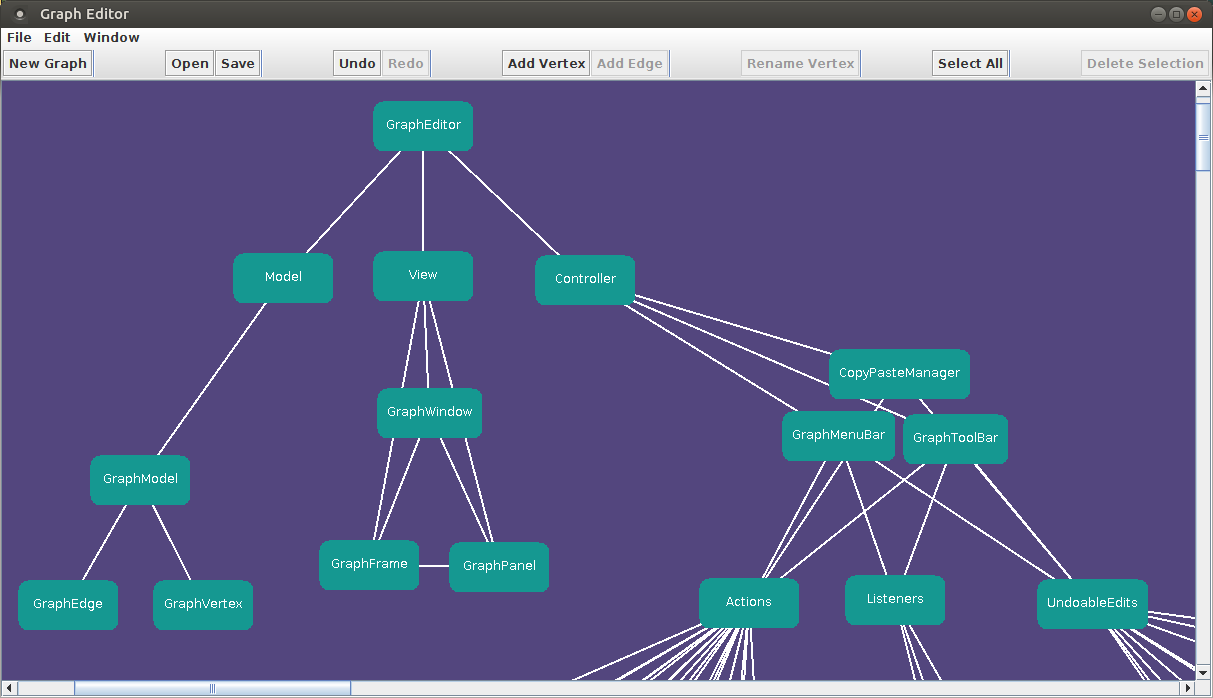
\includegraphics[height=8cm,width=0.95\textwidth]{im/mvc.png}
            \caption{Graph model display in panel}
            \label{fig: mvc}
\end{figure}
\begin{figure}[h!]
            \centering
            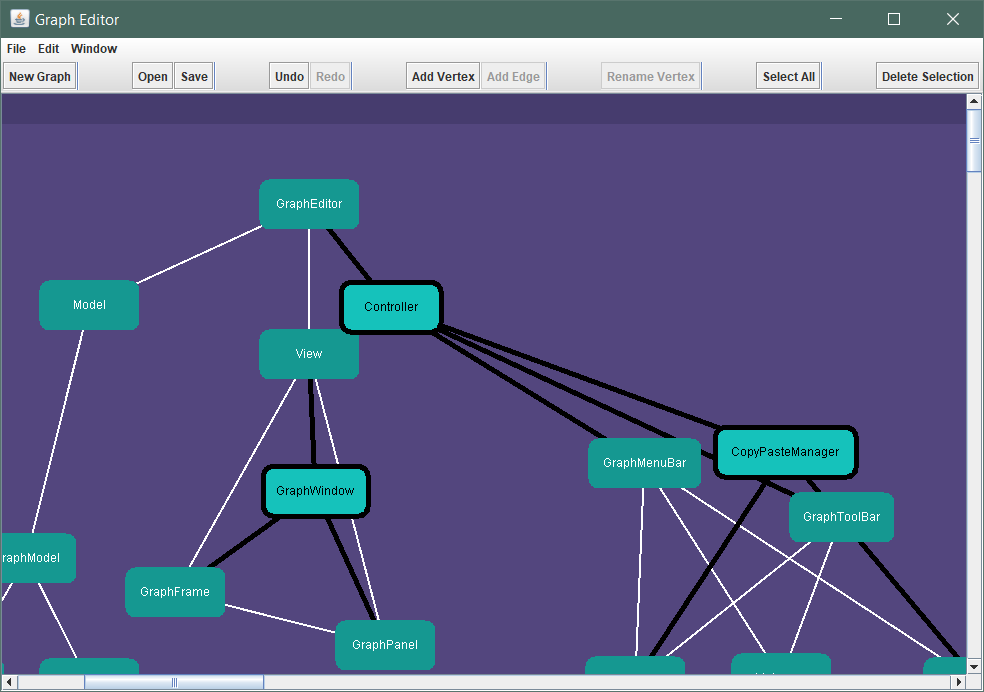
\includegraphics[height=8cm,width=0.95\textwidth]{im/sel.png}
            \caption{Selecting multiple vertices and edges}
            \label{fig: sel}
\end{figure}
\begin{figure}[h!]
            \centering
            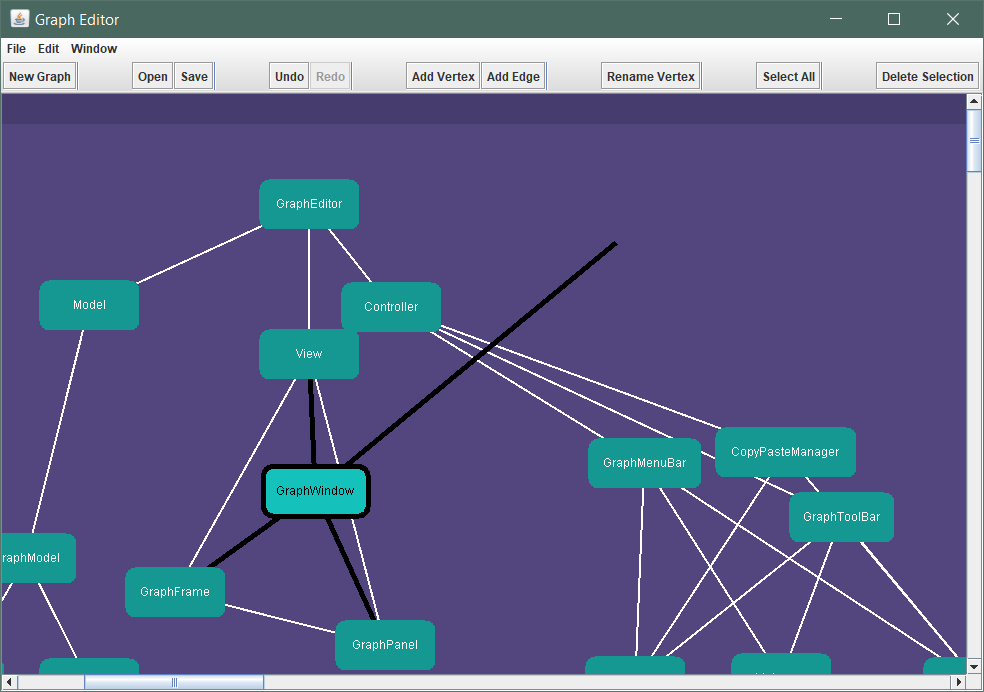
\includegraphics[height=8cm,width=0.95\textwidth]{im/addEdge.png}
            \caption{Adding an edge via the mouse}
            \label{fig: addE}
\end{figure}
\begin{figure}[h!]
            \centering
            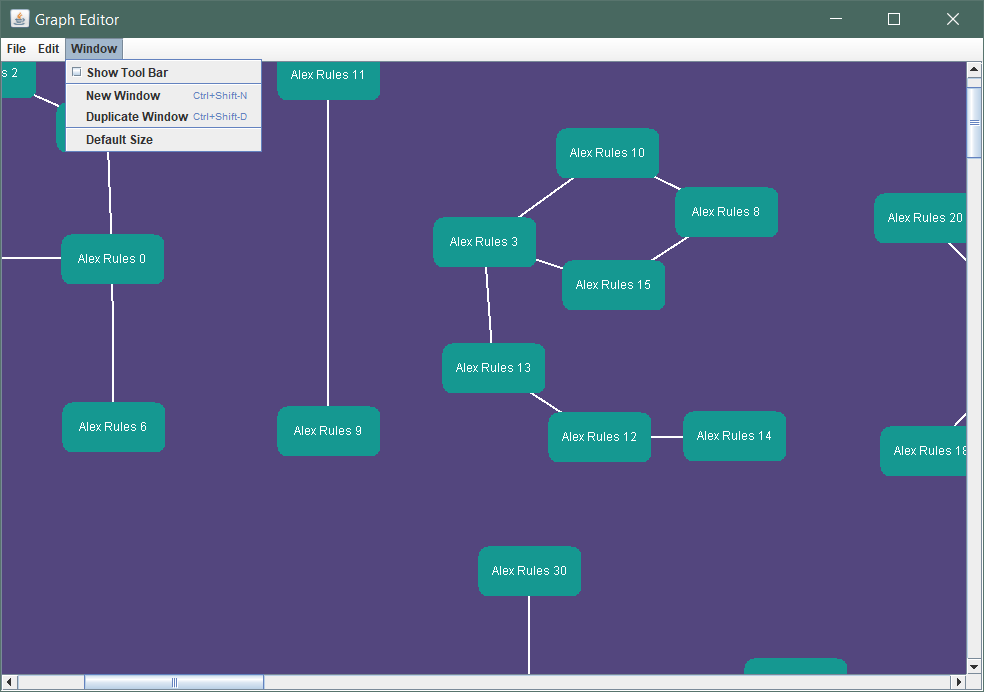
\includegraphics[height=8cm,width=0.95\textwidth]{im/toggled.png}
            \caption{Toggled off tool bar via the menu bar}
            \label{fig: tog}
\end{figure}
\begin{figure}[h!]
            \centering
            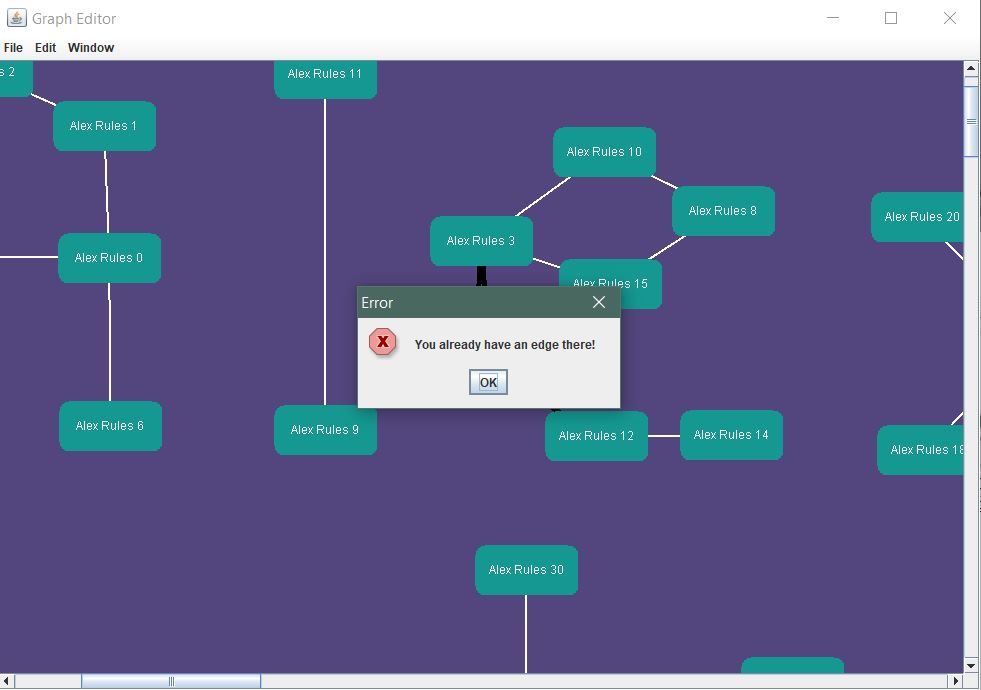
\includegraphics[height=9cm,width=0.95\textwidth]{im/popUpEdge.JPG}
            \caption{Pop up error for adding a clone edge}
            \label{fig: edgePopUp}
\end{figure}
\begin{figure}[h!]
            \centering
            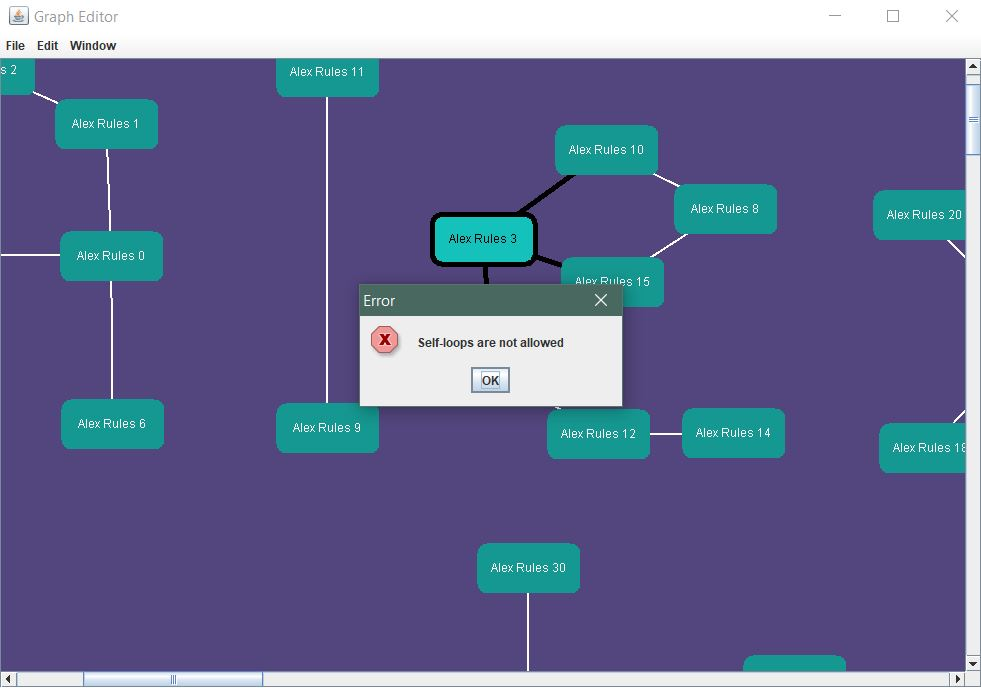
\includegraphics[height=9cm,width=0.95\textwidth]{im/popUpSelfLoop.JPG}
            \caption{Pop up error for connecting a vertex to itself}
            \label{fig: edgeSelfLoop}
\end{figure}
\begin{figure}[h!]
            \centering
            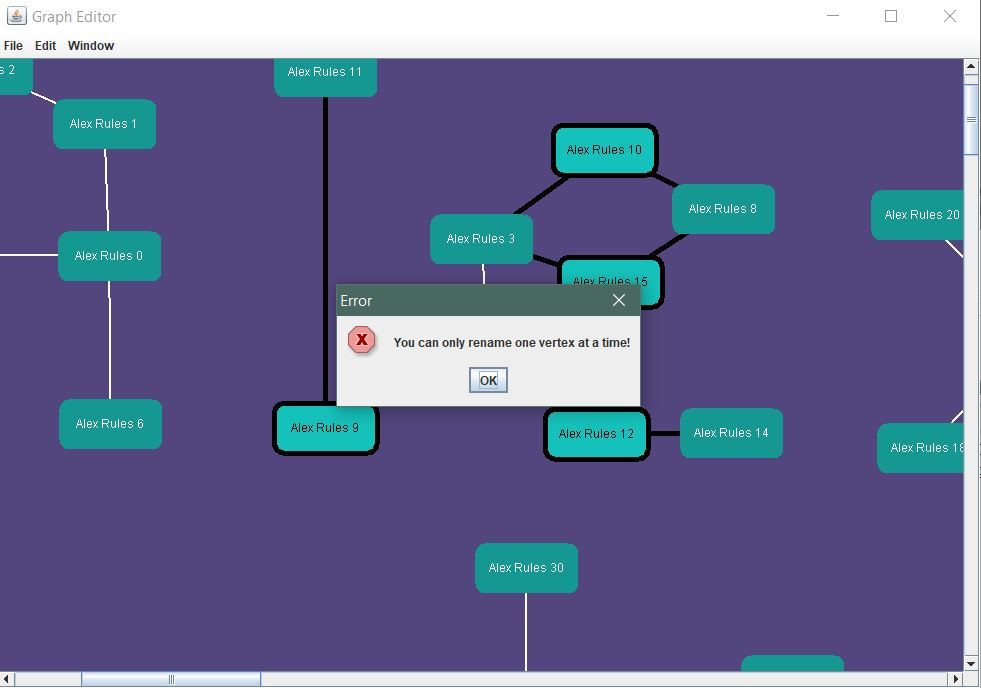
\includegraphics[height=9cm,width=0.95\textwidth]{im/popUpRename.JPG}
            \caption{Pop up error for renaming multiple vertices}
            \label{fig: ErrorRen}
\end{figure}
\begin{figure}[h!]
            \centering
            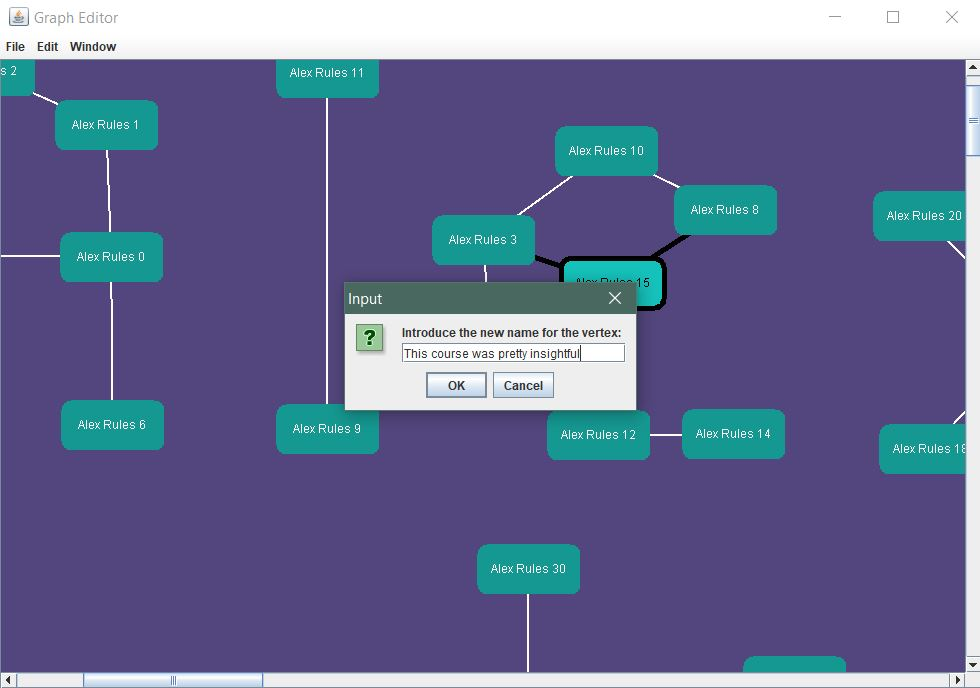
\includegraphics[height=9cm,width=0.95\textwidth]{im/rename.JPG}
            \caption{Renaming a vertex}
            \label{fig: ren}
\end{figure}

\end{document}